% !TeX spellcheck = en_US
\documentclass{article}
\usepackage{graphicx}
\usepackage{hyperref}
\usepackage{float}
\usepackage{multicol}

\title{Practica 2: Algoritmos de Ordenamiento Parte 2}

\author{Adolfo Roman Jimenez}

\begin{document}
	\maketitle
	
	\section{Objetivo}
	El estudiante identificará la estructura de los algoritmos de ordenamiento BubbleSort, QuickSort y	MergeSort
	
	\section{Desarrollo}
	
		\subsection{Ejercicio 1}
		
			\subsubsection{QuickSort}
			
				Antes de comenzar a analizar el algoritmo \emph{QuickSort} se debe de mencionar que este incluye una funcion auxiliar cuyo nombre es \emph{partition().}\\
				
				El algortimo \emph{QuickSort} utiliza 3 argumentos, un arreglo de numeros enteros llamado \textbf{arr} y dos enteros respectivamente que son \textbf{low} y \textbf{high}.\\
				
				Los enteros \textbf{low} y \textbf{high} en realidad corresponden al primero y ultimo indices del arreglo \textbf{arr} insertado, por lo que \textbf{low} siempre sera 0 y \textbf{high} correspondera al tamano del arreglo - 1 unidad.\\
				
				Despues de esto, el codigo en \emph{QuickSort} asigna una variable \textbf{pi} de tipo entero al resultado de la funcion \emph{partition()}.\\
				
				\emph{QuickSort} es un algoritmo que usa la estrategia \emph{"divide y venceras"} y lo que hace en realidad, es que genera algo llamado \emph{pivote} que funciona como referencia para ordenar el arreglo, pues en terminos generales, todo elemento que tenga un valor inferior al pivote lo posiciona en el lado izquierdo y todo elemento que contrariamente tenga un valor superior, lo posicionara en el lado derecho del pivote.\\
				
				En esta version de \emph{QuickSort} el pivote se escoje al final del arreglo, pero existen diferentes versiones del mismo algoritmo donde el pivote puede elegirse al principio, al final o en un punto al azar del arreglo.\\
				
				El programa despues evalua si \textbf{low} es menor a \textbf{high}, si esto es verdadero, entonces declara una variable entera \textbf{pi} que es el punto en donde el arreglo se particionara. El valor de esta variable, es proporcionado por la funcion \emph{paritition()} que devuelve un valor entero.\\
				
				La funcion \emph{partition()} de igual forma que \emph{QuickSort} toma 3 argumentos que se componen de un arreglo de numeros enteros llamado \textbf{arr} y dos enteros respectivamente que de igual manera son \textbf{low} y \textbf{high}.\\
				
				Despues se declara una variable entera \textbf{pivot} que se iguala al valor en ultimo indice de \textbf{arr}, en seguida se declaran las variables enteras \textbf{j} e \textbf{i}, a \textbf{i} se le asigna el valor del indice menor \textbf{low - 1} y a \textbf{j} para efectos de un \emph{for-loop} se le asigna el valor en \textbf{low} que ira sumando en una unidad a \textbf{j} hasta alcanzar el valor en \textbf{high} que es cuando el loop se rompera.\\
				
				Ya dentro del \emph{loop}, en el caso de que el valor de \textbf{arr} en el indice \textbf{j} sea menor o igual al valor en \textbf{pivot} entonces se le sumara 1 a la variable \textbf{i} y se hace un intercambio de valores entre el indice \textbf{i} y el indice \textbf{j} en \textbf{arr}.\\
				
				Al finalizar y salir del \emph{loop} se hace un intercambio entre los valores en los indices \textbf{i + 1} y \textbf{high} en \textbf{arr} y la funcion finaliza retornando el valor en \textbf{i + 1}.\\
				
				Basicamente lo que la funcion \emph{partition()} hace, es que toma el pivote, que es el ultimo elemento en la primera iteracion y coloca todos los elementos menores que el a la izquierda y mayores a la derecha como lo muestra la siguiente imagen.\\
				
				\begin{figure}[H]
					\centering
					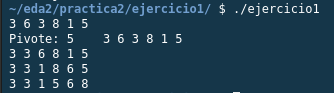
\includegraphics{images/partition1.png}
					\caption{Funcion \emph{partition()} ejecutada sobre arreglo [3, 6, 3, 8, 1, 5]}
				\end{figure} 
			
				Una vez que la variable \textbf{pi} obtiene un valor, se utiliza la recursion obligando a \emph{QuickSort} a invocarse de nuevo, pero esta vez lo hara modificando el valor a \textbf{high} restandole 1, lo que ocasionara que tome como pivote el penultimo digito y repita la operacion recursivamente, lo mismo con una segunda funcion recursiva pero esta vez, el valor en \textbf{low} se traslada a un indice despues de el del pivote, ejecutando la funcion recursivamente de igual forma hasta el momento en que se ordena completamente.\\
				
			
			\subsubsection{BubbleSort}
			
				El algoritmo de \emph{BubbleSort}, como su nombre lo indica, es un algoritmo que va empujando a los numeros mas grandes al final del arreglo donde se encuentran alojados, como si se tratara de una serie de burbujas que se van inflando.\\
				
				El algoritmo de \emph{BubbleSort} es uno muy sencillo, que tiene tambien una implementacion facil, pero que lamentablemente, su tiempo de ejecucion puede llegar a ser de $O(n^2)$ en el peor de los casos.\\
				
				\emph{BubbleSort} comienza tomando 2 argumentos, el primero un arreglo de enteros \textbf{a} y el segundo una variable entera \textbf{size} que corresponde al tamano del arreglo.\\
				
				La funcion declara las variables enteras \textbf{i}, \textbf{j} y \textbf{n}. \textbf{i} y \textbf{j} serviran para iterar en los \emph{loops} subsecuentes mientras que a \textbf{n} se le deposita el valor de \textbf{size}.\\
				
				Cuando comienza a iterar el primer \emph{for-loop} lo hace desde el ultimo indice del arreglo hacia el primero en \textbf{i} y en \textbf{j} inicia desde el 0 hasta el valor en \textbf{i}.\\
				
				En cada iteracion dentro del \emph{for-loop} en \textbf{j} se va evaluando si el numero que se esta revisando es mayor que el siguiente. Si esto es verdadero, entonces el programa intercambia de posicion los numeros y de esta manera el numero mas grande va abriendose paso dentro del arreglo hasta quedar posicionado al final de este, mientras que con cada iteracion los numeros mas chicos, de igual manera se van alejando de la parte derecha del arreglo para llegar a la parte izquierda.\\
				
				El algoritmo finaliza cuando el \emph{for-loop} principal, ha llegado al 0 y es para este tiempo que el arreglo queda ordenado.
				
				
				\subsubsection{BubbleSort - Stop}
				
				Para este ejemplo, lo unico que se me ocurrio fue agregar una especie de \emph{switch} al codigo (y no me refiero a una estructura de control tipo \emph{switch}) en el que creo una variable entera \textbf{x} y le asigno un valor de 1.\\
				
				En el momento en que el algoritmo \emph{BubbleSort} comienza a trabajar, entonces si por lo menos en una ocasion, un numero dentro del arreglo es mayor que el siguiente numero, entonces el valor de \textbf{x} cambia a 0 y el algoritmo continua trabajando mientras.\\
				
				AL finaliar el segundo \emph{for-loop} entonces se encuentra un codigo \emph{if} que evalua si el valor en \textbf{x} es igual o no a 1 y si es igual a 1, entonces quiere decir que el arreglo nunca se modifico, por lo que necesariamente los elementos deben de estar ordenados en forma ascendecente.\\
				
				Si esto sucede entonces la estructura de control rompe el ciclo con un \emph{break} y el programa termina.\\
				
				De esta manera podeos notar que \emph{BubbleSort} cuando el codigo se activa, en una lista ordenada, solamente recorre la lista 1 sola vez, mientras sin el codigo, recorre a lista \textbf{n - 1} veces su longitud aun cuando no existen elementos a modificarse.
				
				\begin{figure}[H]
					\centering
					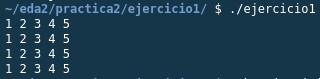
\includegraphics{images/bubblestop1.png}
					\caption{BubbleSort NO modificado, iterando sobre arrelo [1, 2, 3, 4, 5]}
				\end{figure} 
			
				\begin{figure}[H]
					\centering
					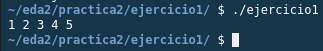
\includegraphics{images/bubblestop2.png}
					\caption{BubbleSort modificado, iterando sobre arrelo [1, 2, 3, 4, 5]}
				\end{figure} 
			
		\subsection{Ejercicio 2}
		
		Agregando la funcion \emph{MergeSort} como estaba en el video e implementandola en \emph{C}, no tuve muchas dificultades para hacerlo. Simplemente tuve que modificar la palabra \emph{list} por un \textbf{int list[]} al momento de escribir los argumentos de las funciones, tanto en \emph{merge()} como en \emph{mergeSort()} y en el caso de \emph{merge()} al momento de crear un segundo arreglo, lo unico que hice fue implementar \textbf{int lista2[r + 1];} que en la nueva version de \emph{C} si es permitido para crear un arreglo con ese numero de posiciones dentro de los barckets cuadrados. 
		
		Al final hice una prueba y ordena correctamente un arreglo que corri con numeros aleatorios.
		
		\begin{figure}[H]
			\centering
			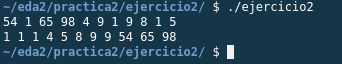
\includegraphics{images/e2.png}
			\caption{Arreglo ordenado con MergeSort}
		\end{figure}
	
		\subsection{Ejercicio 3}
		
		\subsubsection{Menu}
		
		El menu, como el ejercicio lo indica, es el mismo que el de la practica pasada, pero con los nuevos algoritmos integrados a este, de esta forma, tenemos como nuevos elementos del menu a los algoritmos:
		
		\begin{itemize}
			\item \emph{Quick Sort}
			\item \emph{Bubble Sort}
			\item \emph{Merge Sort}
		\end{itemize}
	
		De igual forma, el programa contiene una funcion que realiza un arreglo al azar de los elementos que se deseen y el cual se muestra funcionando en la siguiente imagen:
		
		\begin{figure}[H]
			\centering
			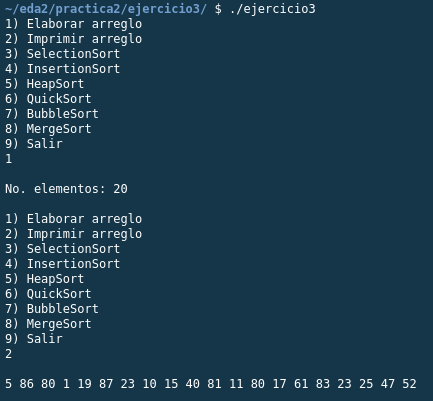
\includegraphics[scale = 0.8]{images/e3menu.png}
			\caption{Menu Principal}
		\end{figure}
		
		\subsubsection{Quick Sort}
		
		La opcion numero 6 corresponde a \emph{QuickSort()} que fue transcrito directamente como venia en la practica. El programa imprime el pivote y los subarreglos que \emph{QuickSort} va generando en cada iteracion.\\
		
		Las imagenes muestran el funcionamiento del programa, primeramete se crear el arreglo al azar de 20 elementos y despues se escoje la opcion numero 6 para que corra el programa.
		
		\begin{figure}[H]
			\centering
			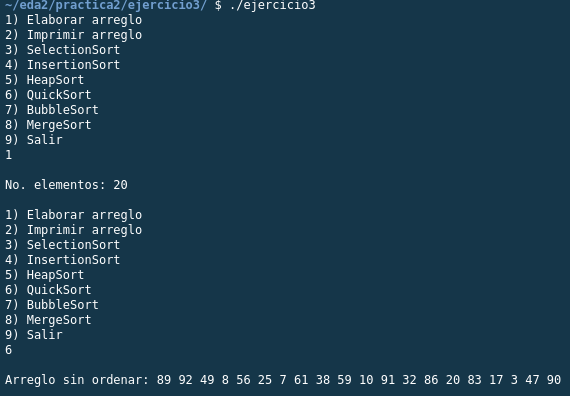
\includegraphics[scale = 0.8]{images/e3q1.png}
			\caption{Funcinamiento QuickSort Imagen 1}
		\end{figure}
	
		\begin{figure}[H]
			\centering
			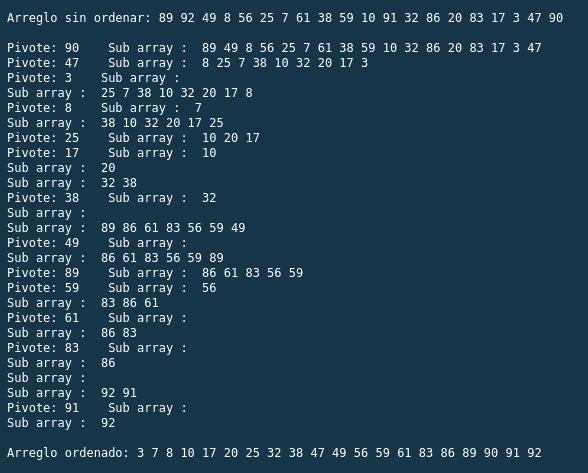
\includegraphics[scale = 0.7]{images/e3q2.png}
			\caption{Funcinamiento QuickSort Imagen 2}
		\end{figure}
	\newpage
		
		\subsubsection{Bubble Sort}
		
		La opcion numero 7 pertenece a \emph{BubbleSort()}. Este programa me gusto mucho como quedo, porque despues de investigar un poco, escribi una funcion alterna \emph{ssswap()} la cual agrega color a los elementos que estan siendo modificados en su posicion en cada iteracion.\\
		
		Las imagenes muestran el funcionamiento del programa, se crea un nuevo arreglo de 20 elementos y al momento de ejecutar el algoritmo, en amarillo se muestra el elemento menor y en verde el elemento que va "arrastrandose" a traves del arreglo hasta que ya no encuentra ningun otro elemento mayor que este, entonces comienza nuevamente al principio del arreglo hasta que termina de ejecutarse.
		
		\begin{figure}[H]
			\centering
			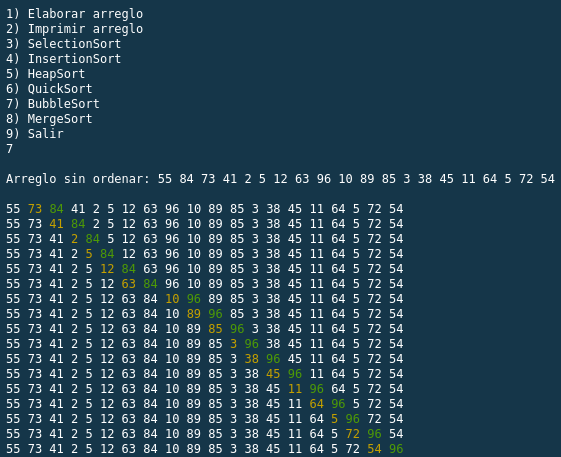
\includegraphics[scale = 0.75]{images/e3b1.png}
			\caption{Algoritmo Bubble Sort Imagen 1}
		\end{figure}
	
		\begin{figure}[H]
			\centering
			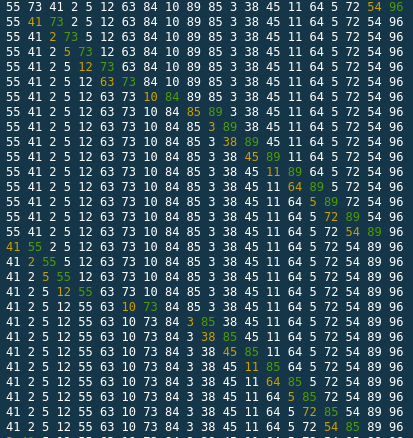
\includegraphics[scale = 1]{images/e3b2.png}
			\caption{Algoritmo Bubble Sort Imagen 2}
		\end{figure}
	
		\begin{figure}[H]
			\centering
			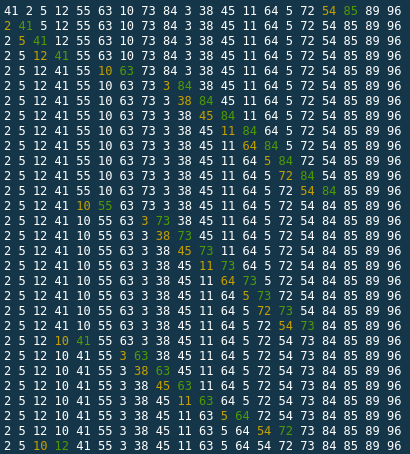
\includegraphics[scale = 1]{images/e3b3.png}
			\caption{Algoritmo Bubble Sort Imagen 3}
		\end{figure}
	
		\begin{figure}[H]
			\centering
			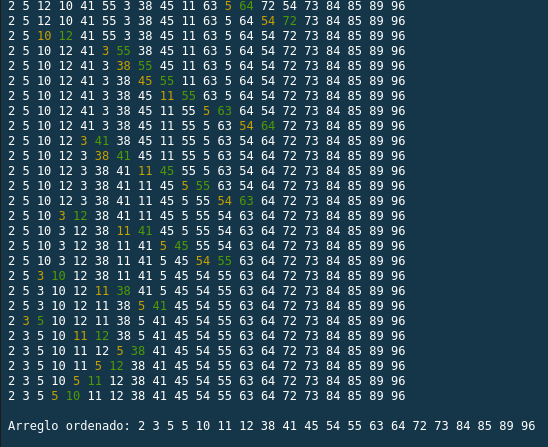
\includegraphics[scale = 0.8]{images/e3b4.png}
			\caption{Algoritmo Bubble Sort Imagen 4}
		\end{figure}
	\newpage
		
		\subsubsection{Merge Sort}
		
		El ultimo algortimo ingresado es \emph{MergeSort()} y sinceramente es un algoritmo \textbf{MUY DIFICIL} de representar a traves de \emph{printf()} como se ejecuta.\\
		
		Una de las cosas que se me ocurrio fue representar los niveles que va generando a traves de su recursion e indicar cuando ingresa a la funcion \emph{merge()} asi como cuando sale de cada una de las funciones recursivas, creo que quedo medianamente comprensible, pero en realidad va generando tantas ramas que es un poco complicado demostrar su funcionamiento si no se utiliza un esquema de arbol para hacerlo.\\
		
		Se incluyen las imagenes de todas formas:
		
		\begin{figure}[H]
			\centering
			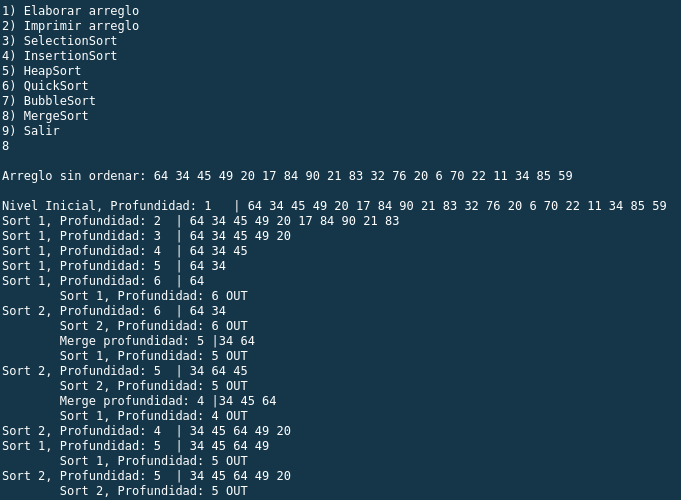
\includegraphics[scale = 0.6]{images/e3m1.png}
			\caption{Funcionamiento Merge Sort Ejemplo 1}
		\end{figure}
	
		\begin{figure}[H]
			\centering
			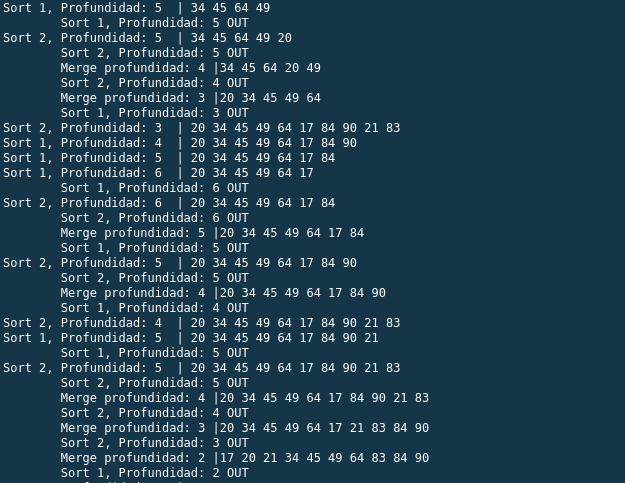
\includegraphics[scale = 0.7]{images/e3m2.png}
			\caption{Funcionamiento Merge Sort Ejemplo 2}
		\end{figure}
	
		\begin{figure}[H]
			\centering
			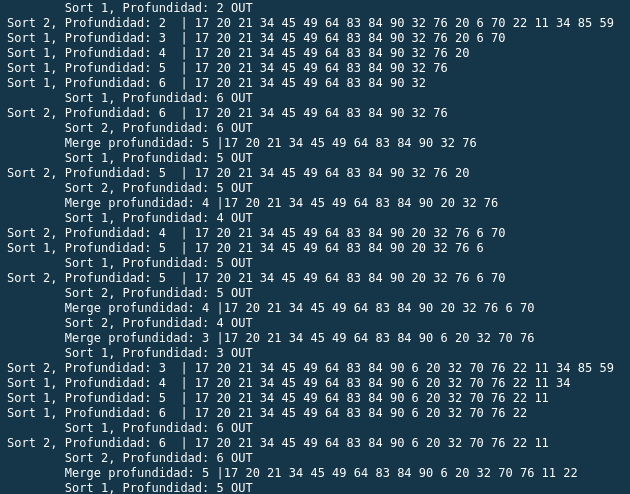
\includegraphics[scale = 0.7]{images/e3m3.png}
			\caption{Funcionamiento Merge Sort Ejemplo 3}
		\end{figure}
	
		\begin{figure}[H]
			\centering
			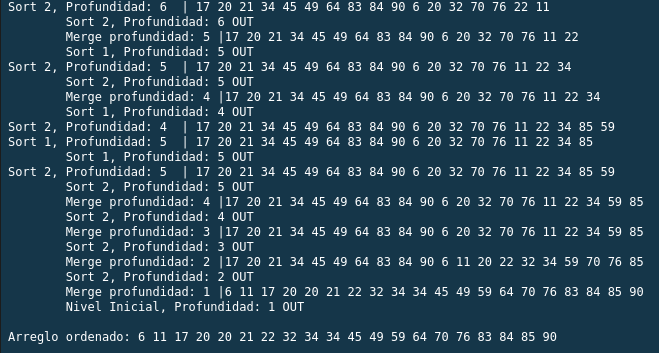
\includegraphics[scale = 0.7]{images/e3m4.png}
			\caption{Funcionamiento Merge Sort Ejemplo 4}
		\end{figure}
	\newpage
				
		\subsection{Ejercicio 4}
		
		Para este ejercicio modifique el codigo que realice en la practica pasada sustituyendo los algoritmos pasados por los nuevos pero ademas agregue algunas modificaciones al codigo de los algoritmos para que se adecuaran a las iteraciones correctas o para que finalizaran sus funciones en caso de que la lista este ordenada.\\
		
		Una de las cosas que se agregaron a \emph{BubbleSort()} por ejemplo, fue un tipo de \emph{switch} que simplemente se activa en caso de que el programa ejecute algun \emph{swap} (pues eso significaria que el algortimo aun no esta del todo ordenado) y en caso de que ningun \emph{swap} se ejecute, entonces el algoritmo tiene instrucciones para que finalice el proceso.\\
		
		De igual forma, agregue instrucciones a \emph{QuickSort()} para que hiciera algo similar. Lo que hice fue que en su funcion \emph{partition()} agregue un contador para que sumara el numero de veces que hace un \emph{swap} y si este numero de veces es igual al tamano del arreglo menos una unidad y ademas el contador \textbf{NO} es igual a 0, entonces el algortmo de igual manera, termina su ejecucion enviando un numero negativo a la funcion principal.\\
		
		Para \emph{MergeSort()} no agregue ningun tipo de funcionalidad para terminar el algoritmo, puesto que basado en el modelo RAM, a pesar de que tiene varios \emph{while-loops} dentro de la funcion \emph{merge()} no se considera que afecten la complejidad temporal del algoritmo.\\
		
		\subsubsection{Graficas de Complejidad}
		
		En general, a excepcion de \emph{MergeSort()} que tiene una complejidad de $O(n log(n))$ practicamente para cualquier caso, los otros 2 algoritmos si sucede que su complejidad temporal es mas alta, especialmente para casos en los que las listas estan organizadas de forma descendente.\\
		
		Como en el ejercicio pasado, se realizaron un total de 45 pruebas que incluyeron arreglos de diferentes tamanos y ordenados tanto de forma ascedente, descendente y aleatoria.\\
		
		Se escogieron estas cantidades numericas principalmente por que se incuyen 3 potencias de 10 (10, 100 y 1000), 1 cantidad intermedia (500) y el doble de la 3ra potencia (2000) pues apartir de esa cantidad las graficas comienzan a crecer muy rapido.\\
		
		Esta es la tabla de resultados generales que obtuve en base a las pruebas que realice:
		
		\begin{figure}[H]
			\centering
			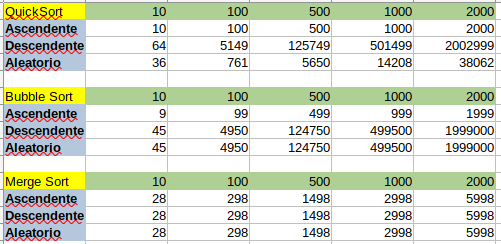
\includegraphics[scale = 0.7]{images/e4t.png}
			\caption{Resultado de suma de ciclos por cantidad de elementos}
		\end{figure}
	\newpage
	
		\subsubsection{Quick Sort}
		
		La grafica de Quick Sort, tiene diferentes resultados cuando trabaja con un arreglo aleatorio, pero cuando se trata de arreglos ascendentes o descendentes, sus ciclos se mantienen constantes.
		
		Se puede apreciar como los arreglos ordenados de forma descendente aumentan de forma exponencial los ciclos que el algoritmo requiere para finalizar su ejecucion. Esto se da probablemente porque en esta version de \emph{QuickSort()} se toma el ultimo elemento como pivote y debido a que en este tipo de arreglos el ultimo elemento es el menor, entonces probablemente es por esa razon que su tiempo de ejecucion aumenta considerablemente. 
		
		\begin{figure}[H]
			\centering
			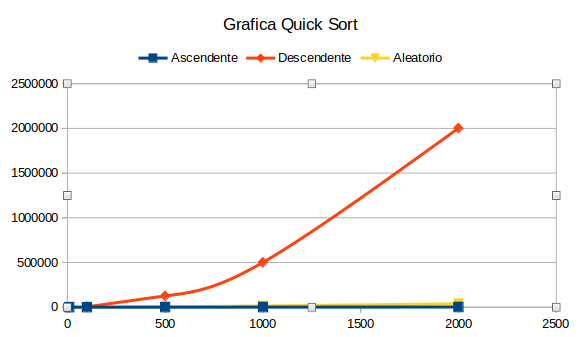
\includegraphics[scale = 0.75]{images/e4gqs.png}
			\caption{Grafica QuickSort, en el eje $x$ se muestran los datos y en el $y$ los ciclos}
		\end{figure}
	\newpage
		
		\subsubsection{Bubble Sort}
		
		En cuanto al algoritmo de \emph{BubbleSort()}, por la forma en la que este se comporta, como su nombre bien lo dice, en forma de "burbuja", unicamente puede llegar al caso de $O(n)$ cuando todos sus elementos estan ordenados de forma ascendente.\\
		
		En cualquier otro caso, el algoritmo tiene un tiempo similar al de $O(n^2)$ siendo en las listas descendentes cuando principalmente se comporta de esta manera, pues al momento de tener al numero menor en el otro extremo del arreglo y al mayor en el extremo inicial, este algoritmo recorre practicamente, $n * n$ veces el arreglo para poder ordenarlo de forma ascendente. \\ 
		
		\begin{figure}[H]
			\centering
			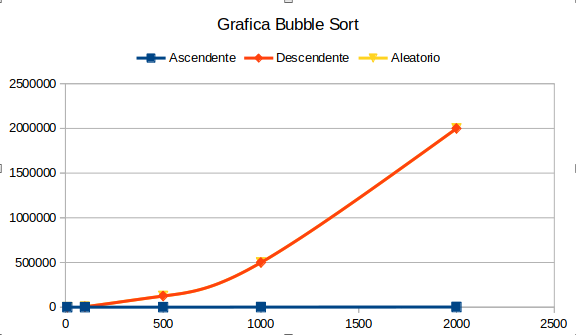
\includegraphics[scale = 0.65]{images/e4gbs.png}
			\caption{Grafica BubbleSort, en el eje $x$ se muestran los datos y en el $y$ los ciclos}
		\end{figure}
	
		\subsubsection{Merge Sort}
		
		\emph{MergeSort()} que se basa en la tecnica \emph{"divide and conquer"} tiene un tiempo estable porque en realidad es un algoritmo que no toma en cuenta los valores del arreglo hasta que se encuentra todo subdividido dentro de las funciones recursivas que ejecuta y es ahi cuando comienza el proceso de arreglo, por lo que \emph{MergeSort()} no es posible limitarlo cuando se le transfiere un arreglo ya ordenado, pues tal vez la unica manera de que \emph{MergeSort()} tuviera una complejidad de $O(n)$ para un arreglo ascendente, seria evaluar el arreglo con anterioridad de forma lineal y asi determinar que no es necesario usar el algoritmo.\\
		
		Esta es basicamente la razon por la que su grafica se ve casi lineal, pues para todos los casos \emph{MergeSort()} hace practicamente lo mismo y el proceso de ordenamiento no se entiende como modificador de la complejidad temporal bajo el modelo \emph{RAM}.
		
		\begin{figure}[H]
			\centering
			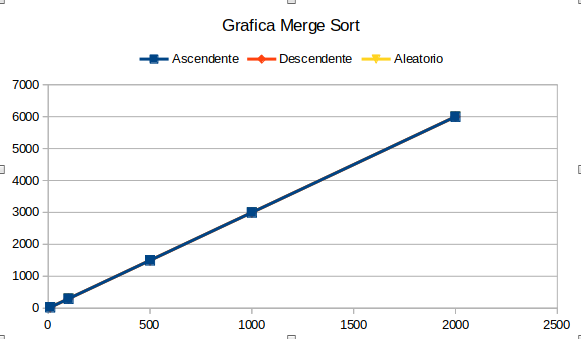
\includegraphics[scale = 0.7]{images/e4gms.png}
			\caption{Grafica MergeSort, en el eje $x$ se muestran los datos y en el $y$ los ciclos}
		\end{figure}
		\newpage
		
		\subsubsection{Output}
		
		Como en la practica pasada, se adjuntan las capturas de pantalla de como se comporto el programa automatizado al momento de ejecutarse.
		
		\begin{figure}[H]
			\centering
			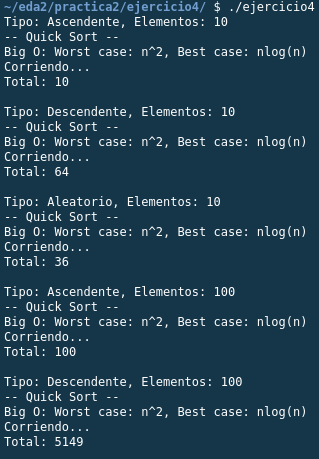
\includegraphics[scale = 1]{images/e41.png}
			\caption{Output programa automarizado}
		\end{figure}
	
		\begin{figure}[H]
			\centering
			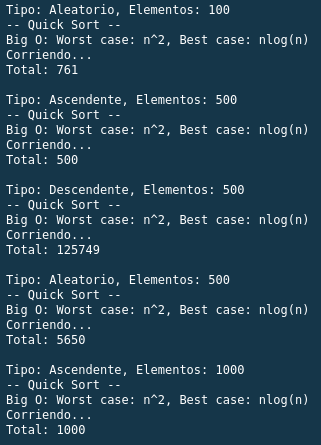
\includegraphics[scale = 1]{images/e42.png}
			\caption{Output programa automarizado}
		\end{figure}
	
		\begin{figure}[H]
			\centering
			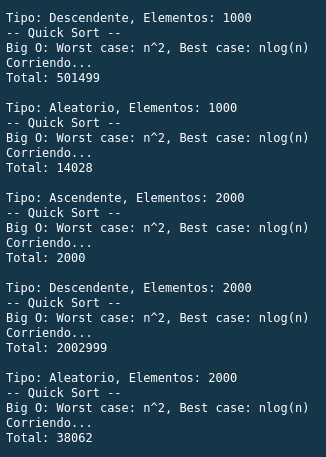
\includegraphics[scale = 1]{images/e43.png}
			\caption{Output programa automarizado}
		\end{figure}
	
		\begin{figure}[H]
			\centering
			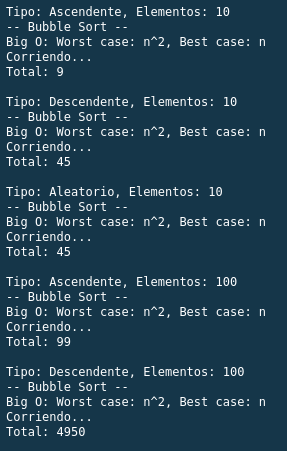
\includegraphics[scale = 1]{images/e44.png}
			\caption{Output programa automarizado}
		\end{figure}
	
		\begin{figure}[H]
			\centering
			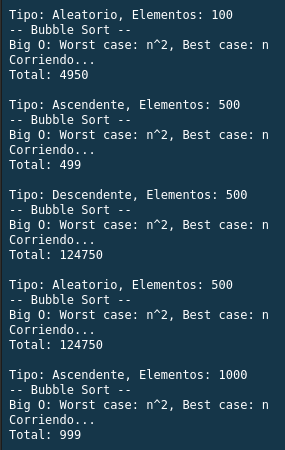
\includegraphics[scale = 1]{images/e45.png}
			\caption{Output programa automarizado}
		\end{figure}
	
		\begin{figure}[H]
			\centering
			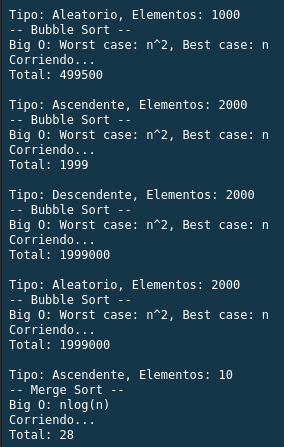
\includegraphics[scale = 1]{images/e46.png}
			\caption{Output programa automarizado}
		\end{figure}
	
		\begin{figure}[H]
			\centering
			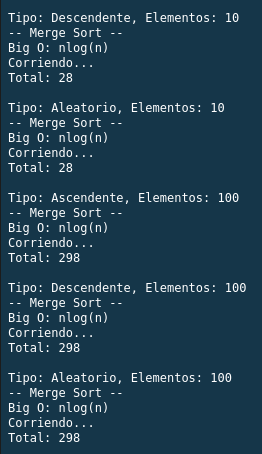
\includegraphics[scale = 1]{images/e48.png}
			\caption{Output programa automarizado}
		\end{figure}
	
		\begin{figure}[H]
			\centering
			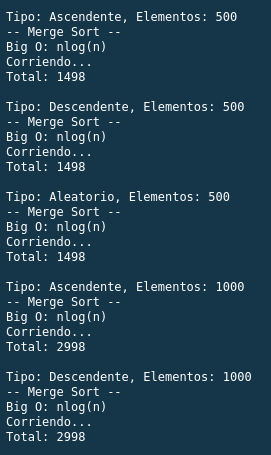
\includegraphics[scale = 1]{images/e49.png}
			\caption{Output programa automarizado}
		\end{figure}
		
		\begin{figure}[H]
			\centering
			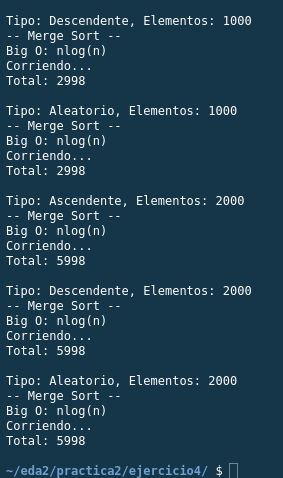
\includegraphics[scale = 1]{images/e410.png}
			\caption{Output programa automarizado}
		\end{figure}
	
		\subsection{Ejercicio 5}
		
		El ejercicio en realidad no se me dificulto, pero si tuve que hacer algunas busquedas principalmente sobre como declarar un arreglo, pues no sabia como se declaraban los arreglos en \emph{Java} pero al estilo de \emph{Java}, que principalmente es una forma diferente a como se hace en \emph{C} y que se escribe de la siguiente manera:\\
		
		int[ ] foo = new int[num];\\
		
		Por otro lado me parece que es la primera ocasion que creo un metodo por mi parte y lo llamo desde otra clase.\\
		
		Una de las cosas que son interesantes en \emph{Java} es que yo suponia que habia que agregar las clases de la misma forma que se hace en \emph{C} con los archivos con extensiones \verb*|.c| o \verb*|.h| que se deben de incluir al principio del documento.\\
		
		Me parecde que con \emph{Java} precisamente por la forma en la que trabaja el \emph{JDK} que basicamente genera un sistema donde todas las clases navegan en el mismo ambiente, pues les es posible interactuar unas con otras ya que dentro del \emph{JDK} de cierta forma se encuentran dentro del mismo \emph{"scope"}.\\
		
		Otra cosa que no me queda aun bien clara, es que no hubo problema en quitar la descripcion \verb*|public| de la clase y funciones dentro del archivo \verb*|Utilidades.java|, pues yo tenia la idea de que si no se indicaba que la clase es publica, entonces no se puede tener acceso a ella. No se si esto sea considerado una buena o mala practica, pues apenas me estoy familiriazando con todo el lenguaje.\\
		
		Por otro lado quisiera aprender mas sobre los \emph{getters} y \emph{setters} que aun no he podido aprender adecuadamente.\\
		
		En general, fuera de investigar como declarar un arreglo, el ejercicio lo hice yo solo y no me parecio especialmente complicada la implementacion.\\
		
		El programa que hice, simplemente declara las clases que se mencionan en la practica y utilizo la clase \emph{Scanner} para obtener 20 numeros enteros de un usuario a traves de un \emph{for-loop} que despues de ser almacenados en un arreglo con capacidad para 20 elementos previamente creado (tampoco sabia que los arreglos en \emph{Java} son dinamicos), utilizo el metodo \emph{.quickSort()} para ordenar esos elementos, invocandolo desde la clase \emph{QuickSort}.\\
		
		Adicionalmente como lo recomienda la practica, tambien agregue la funcionalidad necesaria dentro del metodo \emph{.printSubArray()} perteneciente a la clase \emph{Utilidades} para poder imprimir las iteraciones que genera el metodo \emph{.quickSort()} al momento de ordenar el arreglo creado por el propio usuario.\\
		
		Finalmente, cuando el algoritmo termina de ejecutarse, se imprime como salida a la pantalla y el programa finaliza.\\
		
		A continuacion se adjuntan imagenes de como se ejecuta mi programa:
		
		\begin{figure}[H]
			\centering
			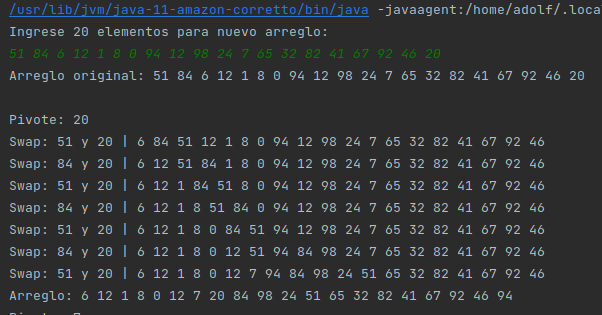
\includegraphics[scale = 0.7]{images/e51.png}
			\caption{Output QuickSort en IntelliJ IDEA}
		\end{figure}
	
		\begin{figure}[H]
			\centering
			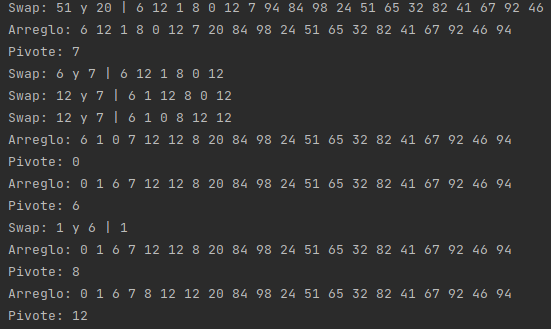
\includegraphics[scale = 0.8]{images/e52.png}
			\caption{Output QuickSort en IntelliJ IDEA}
		\end{figure}
	
		\begin{figure}[H]
			\centering
			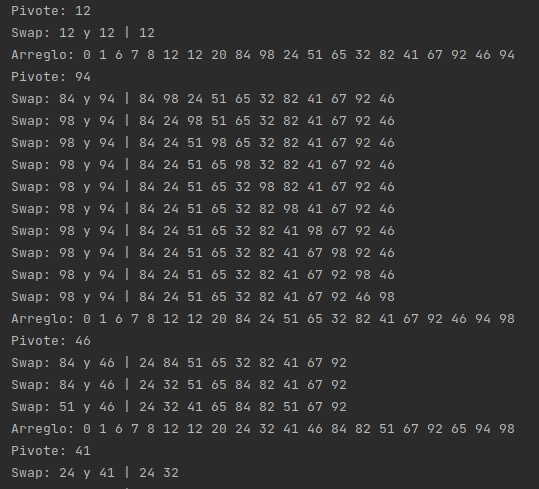
\includegraphics[scale = 0.8]{images/e53.png}
			\caption{Output QuickSort en IntelliJ IDEA}
		\end{figure}

		\begin{figure}[H]
			\centering
			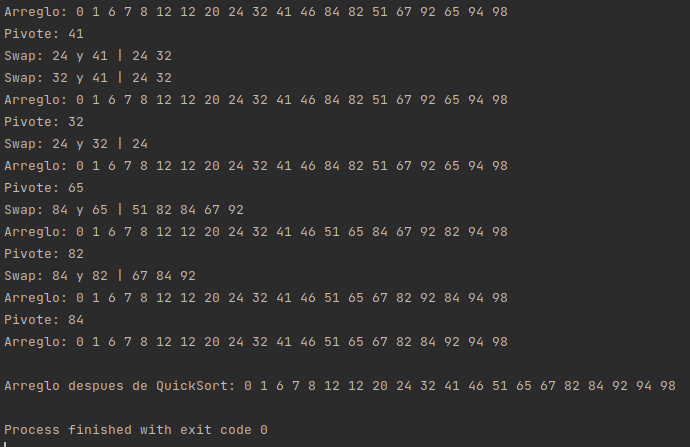
\includegraphics[scale = 0.65]{images/e54.png}
			\caption{Output QuickSort en IntelliJ IDEA}
		\end{figure}
	\newpage		
		
	\section{Conclusiones}
	
	Durante esta practica que fue similar a la pasada, uno de los algoritmos que se me complico un poco fue \emph{Quick Sort} pues su implementacion es un poco confusa y no entendia apropiadamente en que partes realizaba el intercambio de elementos o en que partes no.\\
	
	Una de las partes donde no sabia concretamente que hacer fue al momento que en la funcion \emph{partition()}, el algoritmo lo que evalua es si el elemento en \textbf{j} es menor o igual al pivote y pues al momento evaluar arreglos previamente ordenados, el algoritmo continuaba evaluando valores a pesar de que estos ya estuvieran ordenados, por lo que tuve que idear una forma diferente de poder detener la funcion y ayudarle a determinar el momento en el que un arreglo ya se encuentra ordenado.\\
	
	Para \emph{Bubble Sort} esa parte no me fue tan complicada en realidad, simplemente idee una manera de sencilla de detener las iteraciones del algoritmo siempre y cuando no haya realizado ningun cambio al arreglo sobre el que se ejecutaba lo que significaria que el arreglo entonces ya esta ordenado.\\
	
	Sin embargo para \emph{Merge Sort} lo que me parecio mas complejo fue poder representar alguna forma no tan dificil de imprimir la logica del algoritmo, pues \emph{Merge Sort} genera muchisimas ramificaciones que es dificil representar en una forma lineal.\\
	
	Por otro lado me di cuenta como el modelo \emph{RAM} funciona para casos como el de \emph{Merge Sort}, pues contabilizando todos los ciclos que el algoritmo lleva a cabo para ordenar un arreglo, se puede dar uno cuenta que se transforman en miles para unos cuantos elementos, pero estos ciclos al no estar identados dentro de otros \emph{loops} pues no afectan la complejidad del programa.\\
	
	Con respecto de \emph{Java} aun no me siento del todo familiarizado con el lenguaje y creo que me falta aun mas practica, aunque en realidad la logica de los programas es muy similar. Un profesor de computacion explicaba que para una persona que se dedica de manera profesional al area de la computacion, aprender un nuevo lenguaje es similar a manejar un carro, pues cuando sabes manejar solo es cuestion de un poco de practica manejar el carro que desees pues todos los carros utilizan la misma logica de manejo. Para los lenguajes de programacion la situacion es similar y con \emph{Java}, a pesar de no conocer mucho sobre el lenguaje, tampoco lo siento imposible ni mucho menos, pues una vez que se conoce mas o menos como funciona la logica de los lenguajes de programacion, lo demas es solo cuestion de tiempo y practica.\\
	
	Me gusto mucho la practica y creo que se cumplieron muy bien los objetivos de la clase pues entiendi bastante sobre la implementacion de estos algoritmos, como calcular su complejidad, una de las multiples formas de implementar \emph{Quick Sort} y un poco de \emph{Java}. Espero que pueda pasar a aprender a utilizar estos algoritmos que estuvimos viendo, no solo para ordenar listas de enteros, sino tambien para poder comenzar a usarlos para ordenar archivos o cosas mas complejas que me imagino es en realidad para lo que existen.\\
	
	Para finalizar me da gusto que ya me siento mas fluido en \LaTeX y se me ha facilitado mucho hacer las practicas en este procesador. Ya he aprendido mas sobre como insertar imagenes, insertar codigo, etc y pienso volverme mejor en esto ya que al parecer es una herramienta bastante util.\\
	
	Muchas gracias por leer mi practica!  
	  
	
	
\end{document}